\documentclass{article}
%\usepackage[preprint, nonatbib]{neurips_2020}
\usepackage[nonatbib]{neurips_2020}

\usepackage[utf8]{inputenc}
\usepackage[T1]{fontenc}
\usepackage{amsfonts}
\usepackage{microtype}
\usepackage{hyperref}

\usepackage{booktabs}
\usepackage{graphicx}
\usepackage[square,numbers]{natbib}
\usepackage{makecell}
\usepackage[ruled,vlined]{algorithm2e}
\usepackage{subcaption}
\usepackage{textcomp}
\usepackage{amsthm}
\usepackage{amsmath}

\newtheorem{thm}{Theorem}
\newtheorem{lem}{Lemma}

\renewcommand{\P}{\mathbb{P}}

\title{Supplementary material for MeLES: Metric learning for event sequences with self-supervision}

\author{
Dmitrii Babaev \\
% dmitri.babaev@gmail.com
Sberbank AI Lab
\And
Ivan Kireev \\
Sberbank AI Lab
\And
Nikita Ovsov \\
Sberbank AI Lab
\And
Gleb Gusev \\
Sberbank AI Lab
\And
Maria Ivanova \\
Sberbank AI Lab
\And
Alexander Tuzhilin \\
% \email{atuzhili@stern.nyu.edu}
New York University
}

\begin{document}

\maketitle

\section{Overview}

This is the supplementary material for MeLES: Metric learning for event sequences with self-supervision submission. In Section~\ref{sec-bg} we describe algorithms for batch generation in more details. In Section~\ref{sec-perf-opt} we describe additional optimization tricks for model training and inference. In Section~\ref{sec-proof} we provide the proof for the Theorem 1 from the main paper. In Section~\ref{sec-datasets} we provide more detailed description of the datasets used for experiments. In Section~\ref{sec-exp-setup} we provide additional details about hyper-parameter selection and hand-crafted features design. In Section~\ref{sec-res} we provide visualizations of MeLES embeddings and additional plots for model quality in semi-supervised settings.

\section{Batch generation} \label{sec-bg}

We consider several empirical strategies for sub-sequence generation to compare with random slices algorithm described in section "Sampling of surrogate sequences" of the main paper.
The simplest strategy is the random sampling without replacement.
One more strategy is to produce sub-sequences by random splitting of the initial sequence to several connected segments without intersection between them. To generate k sub-sequences, the following procedure should be repeated k times: take a random number of elements from the sequence \textit{without replacement}.

\begin{algorithm}
\SetAlgoLined
\textbf{hyperparameters:} $k$: number of sub-sequences to be produced. \\
\textbf{input:} A sequence $S$ of length $l$. \\
\textbf{output:} $S_1,...,S_k$: sub-sequences of $S$. \\

\BlankLine
Generate vector $inds$ of length $l$ with random integers from [1,k].\\
 \For{$i\leftarrow 1$ \KwTo $k$}{
 $S_i = S[inds == i]$
 }
\caption{Disjointed sub-sequences generation strategy}
\label{alg-disj-ss}

\end{algorithm}

\section{Performance optimizations} \label{sec-perf-opt}

Here we describe several performance optimizations that can be used for model training and inference.

\textbf{Pair distance calculation.} In order to select negative samples, we need to compute pair-wise distance between all possible pairs of embedding vectors of a batch. For the purpose of making this procedure more computationally effective we perform normalization of the embedding vectors, i.e. project them on a hyper-sphere of unit radius. Since $D(A,B) = \sqrt{\sum_i(A_i - B_i)^2} = \sqrt{\sum_i A_i^2 + \sum_i B_i^2 - 2\sum_i A_i B_i} $ and $||A||= ||B||=1$, to compute the euclidean distance we only need to compute: $\sqrt{2 - 2(A \cdot B)}$.

To compute the dot product between all pairs in a batch we just need to multiply the matrix of all embedding vectors of a batch by itself transposed, which is a highly optimized computational procedure in most modern deep learning frameworks. Hence, the computational complexity of the negative pair selection is $O(n^2h)$ where $h$ is the size of the output embeddings and $n$ is the size of the batch.

\textbf{Embedding update calculation.} Encoder, based on RNN-type architecture like GRU~\cite{Cho2014LearningPR}, allows to calculate embedding $c_{t+k}$ by updating embedding $c_t$ instead of  calculating embedding $c_{t+k}$ from the whole sequence of past events $z_{1:t}$: $c_k = rnn(c_t, z_{t+1:k})$. We use this optimization to reduce inference time to update already existing person embeddings with new events, occurred after the calculation of embeddings. This is possible due to the recurrent nature of RNN-like networks.

\section{Proof of Theorem 1} \label{sec-proof}

In this section, we provide the proof of Theorem 1 that justifies Random Slices sub-sequence generation strategy proposed in the paper. First, we give the statement of Theorem~1 for convenience.

Assume that process $\{X_e(t)\}_{t=1}^{T_e}$ is a segment of a latent process $\{\widehat{X}_e(t)\}_{t=1}^{\infty}$, which generates sequence of all events in the potentially infinite life of entity $e$. That is, we assume that $X_e(t)=\widehat{X}_e(t+s_e)$ for some random starting point $s_e\in \{0,1,\ldots\}$ and horizon $T_e$. Thus we observe, in our data, segment $[s_e+1,s_e+T_e]$ of the life of $e$. We also make the following Assumptions:
\begin{enumerate}
    \item Process $\{\widehat{X}_e(t)\}_{t=1}^{\infty}$ is cyclostationary (in the strict sense)~\cite{Gardner2006Cyclostationarity} with some period $\widehat{T}$.
    \item Starting $s_e$ is independent, and the distribution of $(s_e \mod \widehat{T})$ is uniform over $[0,\widehat{T}-1]$.
    \item Horizon $T_e$ is independent and follows a power--law distribution on $[m,\infty]$.
\end{enumerate}
\begin{thm}\label{thm:distribution}
If sequences $\{x_e(t)\}$ in the dataset are samples of processes $\{X_e(t)\}$, then sub-sequences obtained by the Random Slices generation strategy from $\{x_e(t)\}$ follow the same distribution as $\{x_e(t)\}$ up to a slight alteration of the distribution of the horizon $T_e$. Namely, if $T_e$ follows power law with an exponent $\alpha <-1$, then the density function for the length $T'_e$ of a sub-sequence satisfy 
\begin{equation}\label{probability_ratio}
\P(T'_e=k)/\P(T_e=k)\in \left [\left (\frac{m-1}{m}\right )^{-\alpha},\left (\frac{k}{k-1/2}\right )^{-\alpha}\right ].    
\end{equation}

\end{thm}

\begin{proof}
First, we state the following straightforward lemma:
\begin{lem}\label{stationary}
Let a stochastic process $\{Y(t)\}_{t=1}^{\infty}$ be a shift of another stochastic process $\{\widehat{Y}(t)\}_{t=1}^{\infty}$ by independent random time $s$, i.e. $Y(t) = \widehat{Y}(t+s)$ with integer $s\geq 0$. If process $\{\widehat{Y}(t)\}_{t=1}^{\infty}$ is cyclostationary with period $\widehat{T}$ and $(s_e \mod \widehat{T})$ is uniform over $[0,\widehat{T}-1]$, then process $\{Y(t)\}_{t=1}^{\infty}$ is stationary.
\end{lem}
Lemma~\ref{stationary} implies that process $\{X_e(t)\}_{t=1}^{T_e}$ is stationary, and all its segments $\{X_e(t)\}_{t=s'+1}^{T'_e+s'}$ of a given length $T'_e$ define the same distribution over sequences as its starting segment $\{X_e(t)\}_{t=1}^{T'_e}$ does. Furthermore, integrating over $s'$, we conclude that the conditional distribution of a sub-sequence obtained via Random Slices generation strategy given its length $T'_e$ follows the process $\{X_e(t)\}_{t=1}^{T'_e}$. To finish the proof, it remains to prove Equation~\ref{probability_ratio}.

Assume $\P(T_e=k)\propto k^{\alpha}$ for $k\in [m,\infty]$. By the law of total probability, we have $\P(T'_e=k_0)= \sum_{k}\P(T_e=k)\P(T'_e=k_0\mid T_e=k)$, that is,
$$
\P(T'_e=k_0) = C \sum_{k=k_0}^{\infty} k^{\alpha-1},
$$
where $C$ is the normalization constant. To estimate the sum of the series, notice that
\begin{equation}\label{int_inequal}
\int_{k_0-\frac{1}{2}}^\infty x^{\alpha-1} dx > \sum_{k=k_0}^{\infty} k^{\alpha-1} > \int_{k_0}^\infty x^{\alpha-1} dx,    
\end{equation}
where the former inequality follows from the fact that $\int_{k-1/2}^{k+1/2} x^{\alpha-1}> k^{\alpha-1}$ as long as function $f(x)=x^{\alpha-1}$ is convex. After integration, we rewrite Equation~\ref{int_inequal} as follows:
\begin{equation}\label{inequal}
\frac{-1}{\alpha} \left ( k_0-\frac{1}{2}\right )^{\alpha} > \sum_{k=k_0}^{\infty} k^{\alpha-1} > \frac{-1}{\alpha} k_0^{\alpha}. \end{equation}
Using these inequalities, we obtain the upper bound for $\P(T'_e=k)/\P(T_e=k)$ in the following way:
\begin{multline*}
\P(T'_e=k_0) = \sum_{k=k_0}^{\infty} k^{\alpha-1} / \sum_{l=m}^\infty \sum_{k=l}^{\infty} k^{\alpha-1} < \frac{-1}{\alpha} \left ( k_0-\frac{1}{2}\right )^{\alpha} / \sum_{l=m}^\infty \frac{-1}{\alpha} l^{\alpha} = \\
=\left (\frac{k_0}{k_0-1/2}\right )^{-\alpha} k_0^\alpha/\sum_{l=m}^\infty l^{\alpha} = \left (\frac{k_0}{k_0-1/2}\right )^{-\alpha} \P(T_e=k_0).
\end{multline*}
At last, the lower bound for $\P(T'_e=k)/\P(T_e=k)$ can be obtained using Equation~\ref{inequal} as follows:
\begin{multline*}
\P(T'_e=k_0) = \sum_{k=k_0}^{\infty} k^{\alpha-1} / \sum_{l=m}^\infty \sum_{k=l}^{\infty} k^{\alpha-1} > k_0^{\alpha} / \sum_{l=m}^\infty  \left (l-\frac{1}{2}\right )^{\alpha} > \\
> \left (\frac{m-1/2}{m}\right )^{-\alpha} k_0^\alpha/\sum_{l=m}^\infty l^{\alpha} = \left (\frac{m-1/2}{m}\right )^{-\alpha} \P(T_e=k_0).
\end{multline*}
The latter inequality in these calculations follows from the fact that $\left (\frac{l-\frac{1}{2}}{l}\right )^{\alpha}<\left (\frac{m-\frac{1}{2}}{m}\right )^{\alpha}$ for $l>m$.

\end{proof}

\section{Datasets} \label{sec-datasets}

We designed the method specially for the user behavior sequences~\cite{Ni2018PerceiveYU}. That sequences consist of discrete events per person in continuous time, for example,  behavior on websites, credit card transactions, etc. 

Considering credit card transactions, each transaction have a set of attributes, either categorical or numerical including the timestamp of the transaction. An example of the sequence of three transactions with their attributes is presented in the Table \ref{tab-tr-data}.
Merchant type field represents the category of a merchant, such as "airline", "hotel", "restaurant", etc.

\begin{table}
\centering
\caption{Data structure for a single credit card}
\begin{tabular}{llllll}
\toprule
\textbf{Date} & \textbf{Time} & \textbf{Amount} & \textbf{Currency} & \textbf{Country} & \textbf{Merchant Type} \\
\midrule
Jun 21 & 16:40& 230 & EUR & France & Restaurant \\
Jun 21 & 20:15 & 5 & USD & US & Transportation \\
Jun 22 & 09:30 & 40 & USD & US & Household Appliance \\
\bottomrule
\end{tabular}
\label{tab-tr-data}
\end{table}

Another example of user behavior data is click-stream: the log of internet pages  visits. The example of a click-stream log of a single user is presented in Table \ref{tab-cs-data}.

\begin{table}
\centering
\caption{Click-stream structure for a single user}
\begin{tabular}{llll}
\toprule
\textbf{Time} & \textbf{Date} & \textbf{Domain} & \textbf{Referrer Domain} \\
\midrule
17:40 & Jun 21 & amazon.com & google.com \\
17:41 & Jun 21 & amazon.com & amazon.com \\
17:45 & Jun 21 & en.wikipedia.org & google.com \\
\bottomrule
\end{tabular}
\label{tab-cs-data}
\end{table}


In our research we chose several publicly available datasets from data science competitions.
\begin{enumerate}
    \item \textbf{Age group prediction competition}\footnote{https://onti.ai-academy.ru/competition} - the task is to predict the age group of a person. The dataset consists of 44M anonymized transactions representing 50k persons with a target labeled for only 30k of them (27M out of 44M transactions), for the other 20k persons (17M out of 44M transactions) label is unknown. Each transaction includes date, type (for example, grocery store, clothes, gas station, children's goods, etc.) and amount. We use all available 44M transactions for metric learning, excluding 10\% - for the test part of the dataset, and  5\% for the metric learning validation.
        
    \item \textbf{Gender prediction competition}\footnote{https://www.kaggle.com/c/python-and-analyze-data-final-project/} - the task is a classification problem of predicting a gender. The dataset consists of 6,8M anonymized card transactions representing 15k clients, where only 8,4k of them are labeled. Each transaction is characterized by date, type (for ex. "ATM cash deposit"), amount and Merchant Category Code (MCC).
    
    \item \textbf{Assessment prediction competition}\footnote{https://www.kaggle.com/c/data-science-bowl-2019} - the task is to predict the in-game assessments results based on the history of children gameplay data. The dataset consists of 12M gameplay events representing 4,6k children. Each gameplay event is characterized by timestamp, event code, incremental counter of events within a game session, time since the start of the game session, etc.
    
    \item \textbf{Retail purchase history age group prediction}\footnote{https://ods.ai/competitions/x5-retailhero-uplift-modeling} - the task is to predict the age group of a client based on it retail purchase history. The dataset consists of ???M retail purchases representing ???k clients. Each purchase is characterized by time, product level, segment, amount, value, points received.

\end{enumerate}

\section{Experiment setup} \label{sec-exp-setup}

For all methods, random search on 5-fold cross-validation over the train set is used for hyper-parameter selection. The hyper-parameters with the best out-of-fold performance on train set are then chosen. The final set of hyper-parameters used for MeLES is shown in Table \ref{tab-hyper}.

\begin{table}
\centering
\caption{Hyper-parameters for MeLES training}
\begin{tabular}{lllllll}
\toprule
\textbf{Dataset} & \makecell[l]{\textbf{Learning} \\ \textbf{rate}} & \makecell[l]{\textbf{N samples} \\ \textbf{in batch}} & \textbf{N epochs} & \makecell[l]{\textbf{N} \\ \textbf{sub-samples}}} & \makecell[l]{\textbf{Min seq} \\ \textbf{length}} & \makecell[l]{\textbf{Max seq} \\ \textbf{length}} \\
\midrule
\textbf{Age group} & 0.002 & 64 & 100 & 5 & 25 & 100 \\
\textbf{Gender} & 0.002 & 128 & 150 & 5 & 25 & 100 \\
\textbf{Assessment} & 0.002 & 256 & 100 & 5 & 100 & 500 \\
\textbf{Retail} & 0.002 & 256 & 30 & 5 & 30 & 180 \\
\bottomrule
\end{tabular}
\label{tab-hyper}
\end{table}

\subsection{Hand-crafted features}

Here we describe the the details of producing hand-crafted features. All attributes of each transaction are either numerical (e. g. amount) or categorical (e.g. merchant type (MCC code), transaction type, etc.). 
For numerical type of attribute we apply aggregation functions, such as 'sum', 'mean', 'std', 'min', 'max', over all transactions per user. For example, if we apply 'sum' for the numerical field 'amount' we obtain a feature 'sum of all transaction amounts per user'. 
For categorical type of attribute we apply aggregation functions in a slightly different way. For each unique value of categorical attribute we apply aggregation functions, such as 'count', 'mean', 'std' over all transactions per user' numerical attribute. For example, if we apply 'mean' for the numerical attribute 'amount' grouped by categorical attribute 'mcc code' we obtain a feature 'mean amount of all transaction for each mcc code per user'. 
For example, for age prediction task we have one categorical attribute (small group) with 200 unique values, combining it with amount we can produce $200 * 3$ features ('group0 x amount x count',  'group1 x amount x count', ..., 'group199 x amount x count', 'group0 x amount x mean', ...). In total we use approx 605 features for age prediction task. For gender prediction task we have two categorical features: 'MCC code' with approx 200 unique values and 'tr type' with approx 100 unique values. So in total we use $200 * 3 + 100 * 3 + 5 = 905$ features.
Note, that hand-crafted features contain information about user spending profile but omit information about transactions temporal order.

\subsection{Design choices}

In the Table \ref{tab-enc-type} and Table \ref{tab-loss-type} we present the results of experiments on different design choices of our method.

As shown in Table \ref{tab-enc-type}, different choices of encoder architectures show comparable performance on the downstream tasks.

It is interesting to observe that even contrastive loss that can be considered as the basic variant of metric learning loss allows to get strong results on the downstream tasks (see Table \ref{tab-loss-type}). Our hypothesis is that an increase in the model performance on metric learning task does not always lead to an increase in performance on downstream tasks.

\begin{table}
\centering
\caption{Comparison of encoder types}
\begin{tabular}{llll}
\toprule
\textbf{Dataset} & \textbf{LSTM} & \textbf{GRU} & \textbf{Transformer} \\
\midrule
\textbf{Age group} \small{(Accuracy)} & 0.616 $\pm 0.006$ & \textbf{0.642} $\pm 0.004$ & $0.633 \pm 0.007$ \\
\textbf{Gender} \small{(AUROC)} & $0.866 \pm 0.003$ & \textbf{0.882} $\pm 0.002$ & $0.864 \pm 0.004$  \\
\textbf{Assessment} \small{(Accuracy)} & $0.601 \pm 0.003$ & \textbf{0.604} $\pm 0.003$ & $0.542 \pm 0.002$  \\
\textbf{Retail} \small{(Accuracy)} & $0.540 \pm 0.001$ & \textbf{0.542} $\pm 0.002$ & $0.503 \pm 0.001$  \\
\bottomrule
\end{tabular} \\
\small{5-fold cross-validation metric $\pm 95\%$ is shown}
\label{tab-enc-type}
\end{table}

\begin{table}
\centering
\caption{Comparison of metric learning losses}
\begin{tabular}{llllll}
\toprule
\textbf{Dataset} & \textbf{Contrastive} & \makecell{\textbf{Binomial} \\ \textbf{deviance}} & \textbf{Histogram} & \textbf{Margin} & \textbf{Triplet} \\
\midrule
\makecell{\textbf{Age group} \\ \small{(Accuracy)}} & \makecell{\textbf{0.642} \\ $\pm 0.004$} & \makecell{0.626 \\ $\pm 0.005$} & \makecell{0.629 \\ $\pm 0.004$} & \makecell{0.635 \\ $\pm 0.006$} & \makecell{0.637 \\ $\pm 0.002$} \\
\makecell{\textbf{Gender} \\ \small{(AUROC)}} & \makecell{\textbf{0.881} \\ $\pm 0.004$} & \makecell{0.861 \\ $\pm 0.004$} & \makecell{0.866 \\ $\pm 0.004$} & \makecell{\textbf{0.882} \\ $\pm 0.002$} & \makecell{0.860 \\ $\pm 0.005$} \\
\makecell{\textbf{Assessment} \\ \small{(Accuracy)}} & \makecell{\textbf{0.604} \\ $\pm 0.003$} & \makecell{0.576 \\ $\pm 0.004$} & \makecell{\textbf{0.608} \\ $\pm 0.001$} & \makecell{0.593 \\ $\pm 0.002$} & \makecell{0.601 \\ $\pm 0.003$} \\
\makecell{\textbf{Retail} \\ \small{(Accuracy)}} & \makecell{\textbf{0.542} \\ $\pm 0.002$} & \makecell{0.538 \\ $\pm 0.002$} & \makecell{0.538 \\ $\pm 0.001$} & \makecell{\textbf{0.546} \\ $\pm 0.002$} & \makecell{0.536 \\ $\pm 0.002$} \\
\bottomrule
\end{tabular} \\
\small{5-fold cross-validation metric $\pm 95\%$ is shown}
\label{tab-loss-type}
\end{table}

Figure \ref{fig-emb-dim} shows that the performance quality on the downstream task increases with dimensional of an embedding. As we can see the plots for different datasets have similar shape with significant drop after reaching the peak. As mentioned in the section "Design choices" of the main paper the possible reason of this drop is overfitting, i. e. embedding dimension does not serve as effective information bottleneck.

\begin{figure}
  \centering
  \caption{Embedding dimensionality vs. quality}
  \begin{subfigure}{0.5\linewidth}
    \caption{Age group prediction}
    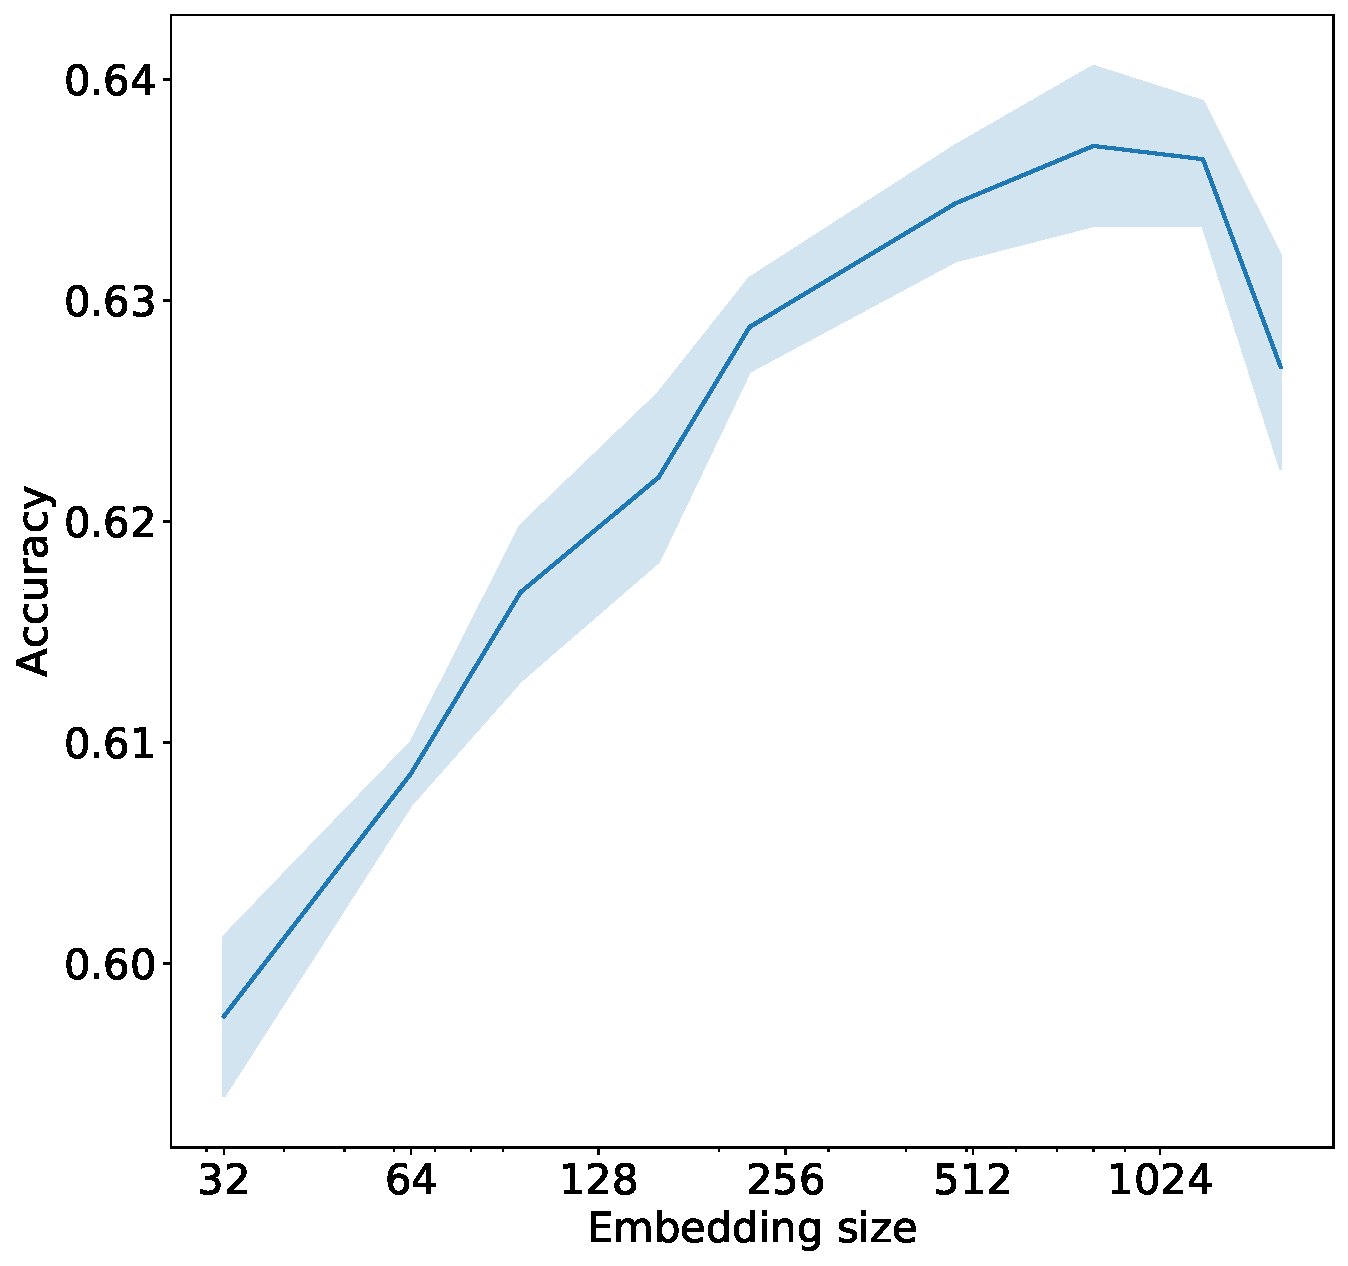
\includegraphics[width=\linewidth]{figures/age-pred-hidden-size.pdf}
    \label{fig-emb-dim-age}
  \end{subfigure}%
  \begin{subfigure}{0.5\linewidth}
    \caption{Gender prediction}
    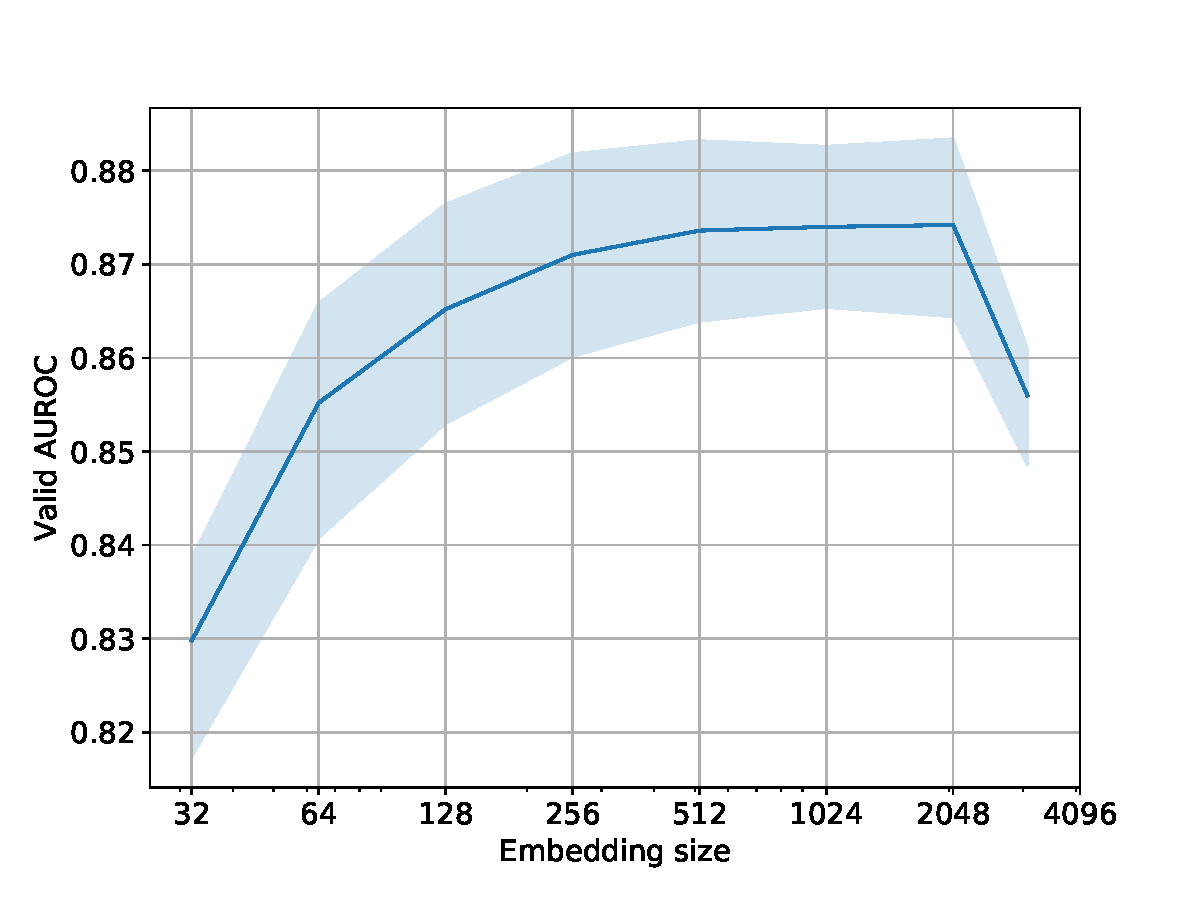
\includegraphics[width=\linewidth]{figures/gender-hidden-size.pdf}
    \label{fig-emb-dim-gender}
  \end{subfigure}
  \begin{subfigure}{0.5\linewidth}
    \caption{Assessment prediction}
    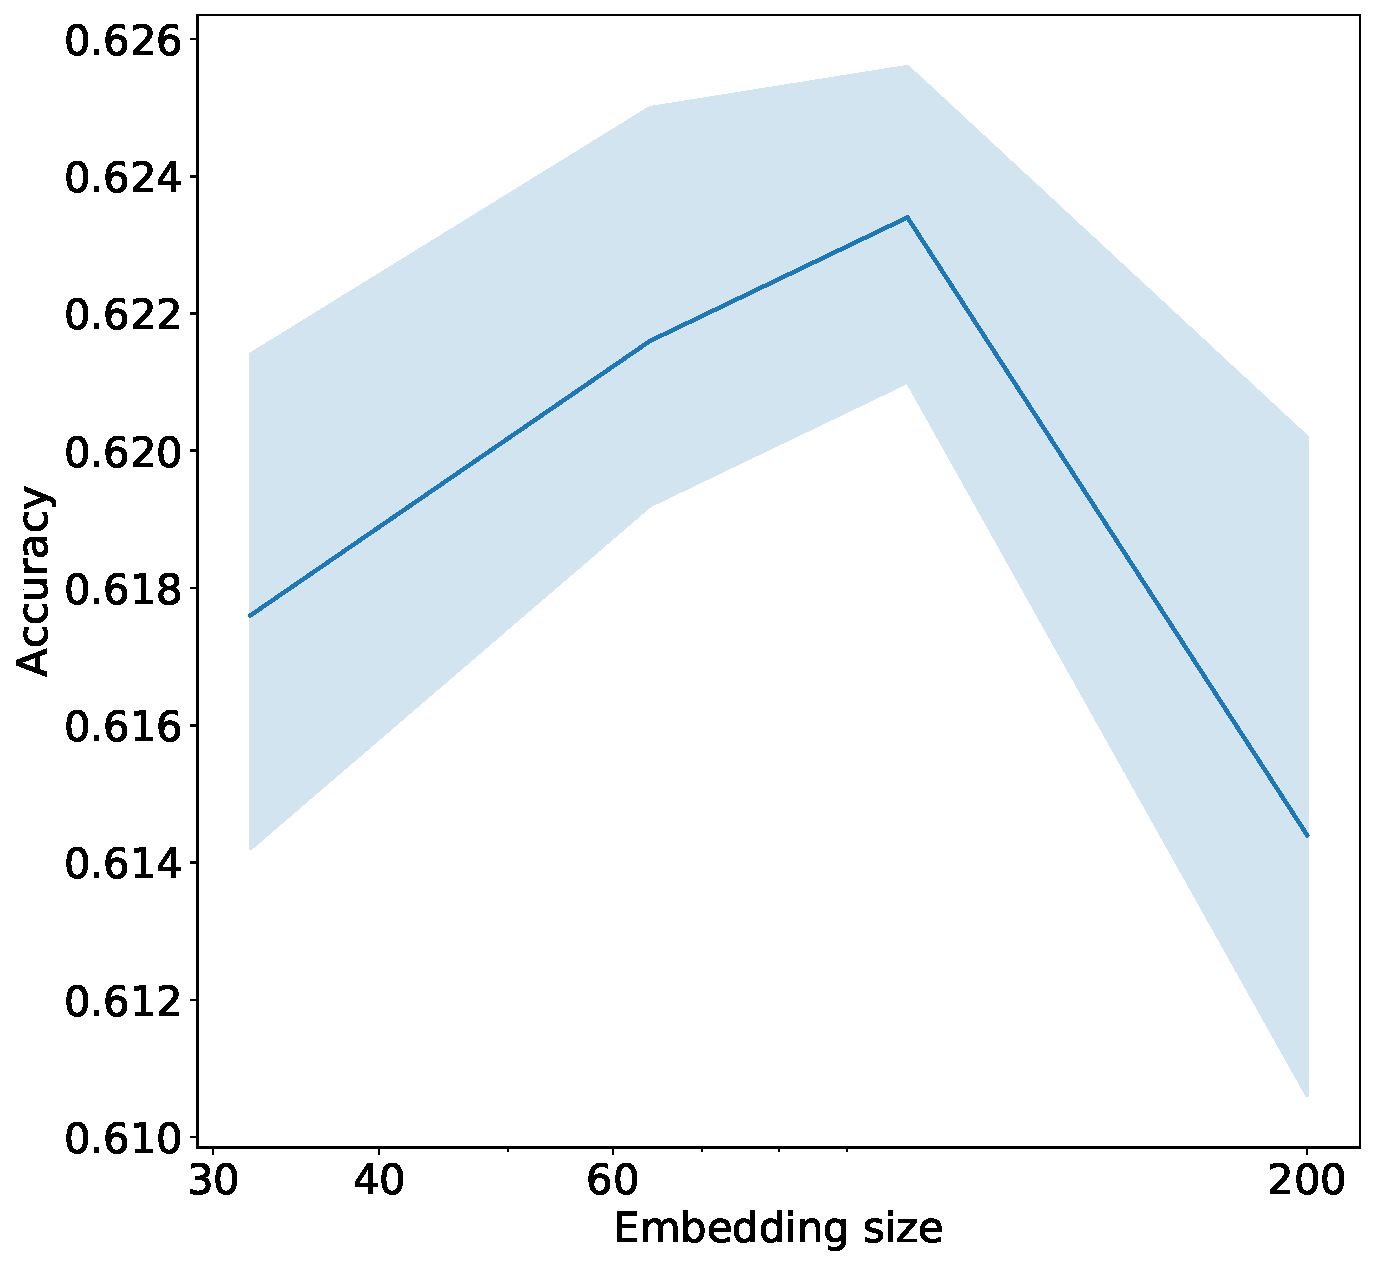
\includegraphics[width=\linewidth]{figures/bowl-hidden-size.pdf}
    \label{fig-emb-dim-bowl}
  \end{subfigure}%
  \begin{subfigure}{0.5\linewidth}
    \caption{Retail prediction}
    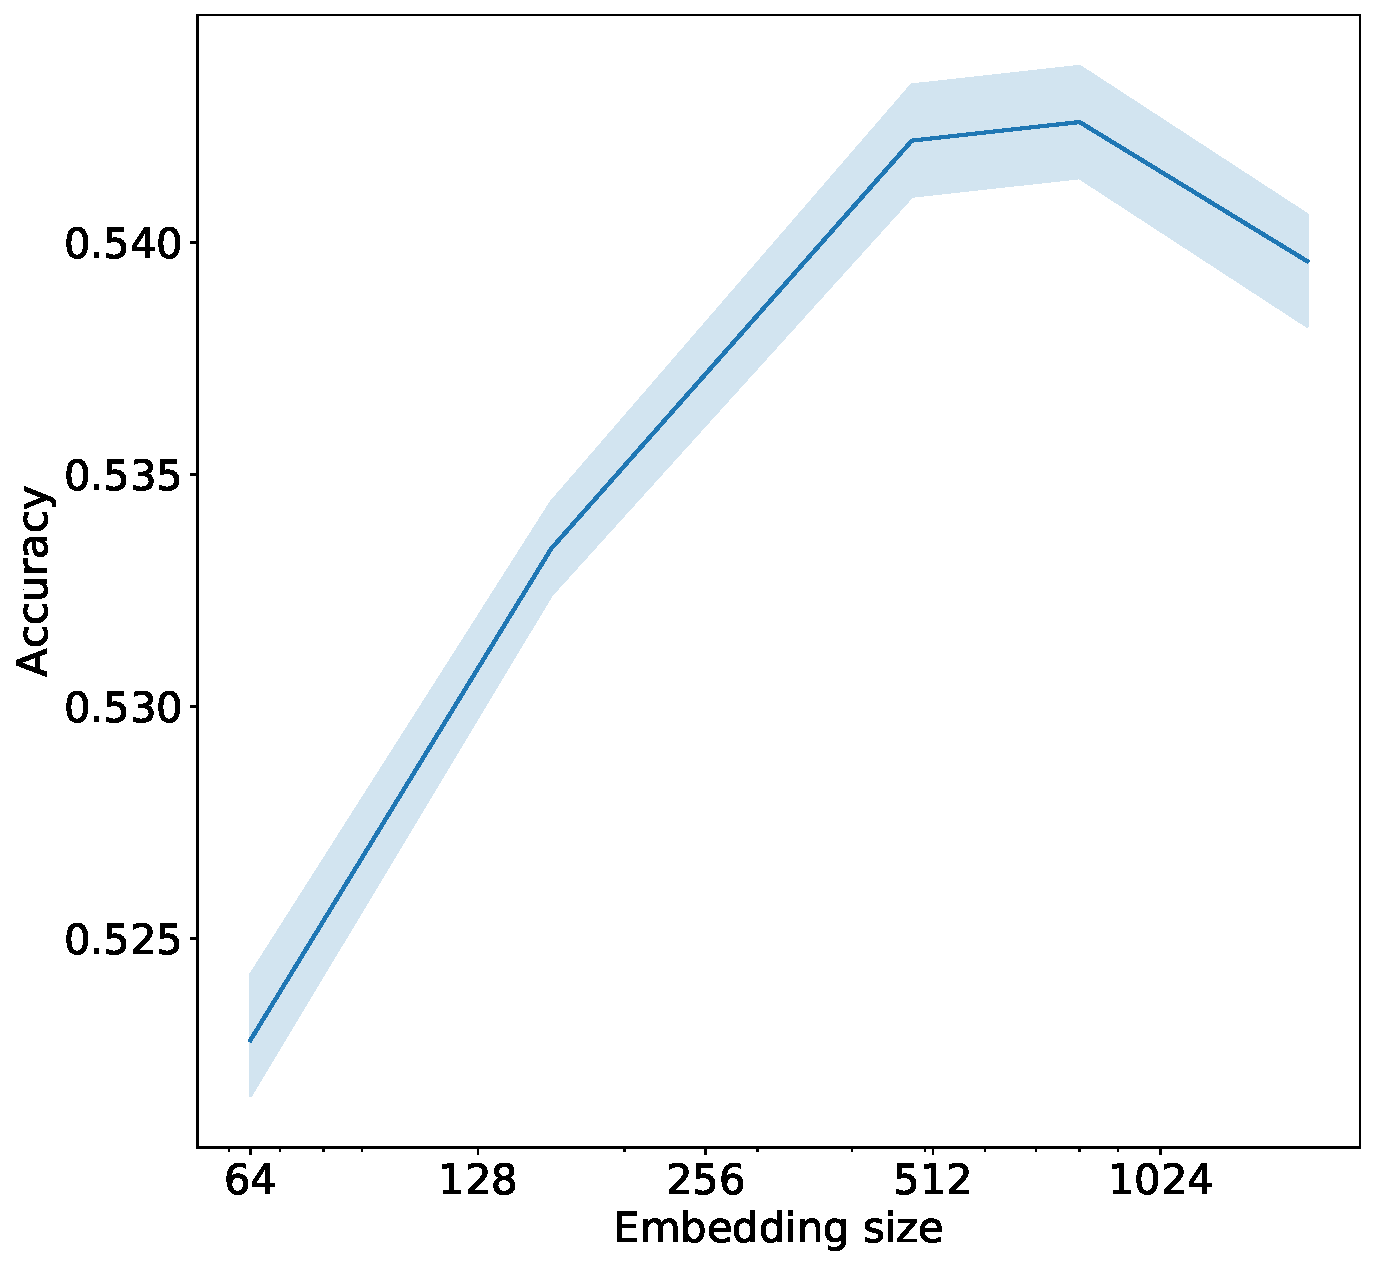
\includegraphics[width=\linewidth]{figures/x5-hidden-size.pdf}
    \label{fig-emb-dim-x5}
  \end{subfigure}
  \label{fig-emb-dim}
\end{figure}

\section{Results} \label{sec-res}

\subsection{Semi-supervised setup}

To evaluate our method in case of the restricted amount of labeled data, we use only part of the available target labels for the semi-supervised experiment. As in the case of the supervised setup, we compare the proposed method with LigthGBM over hand-crafted features, CPC, and supervised learning without pre-training. In figure \ref{fig-semi} we provide learning curves for all considered datasets.

\begin{figure}
  \centering
  \begin{subfigure}{0.5\linewidth}
    \caption{Age group prediction}
    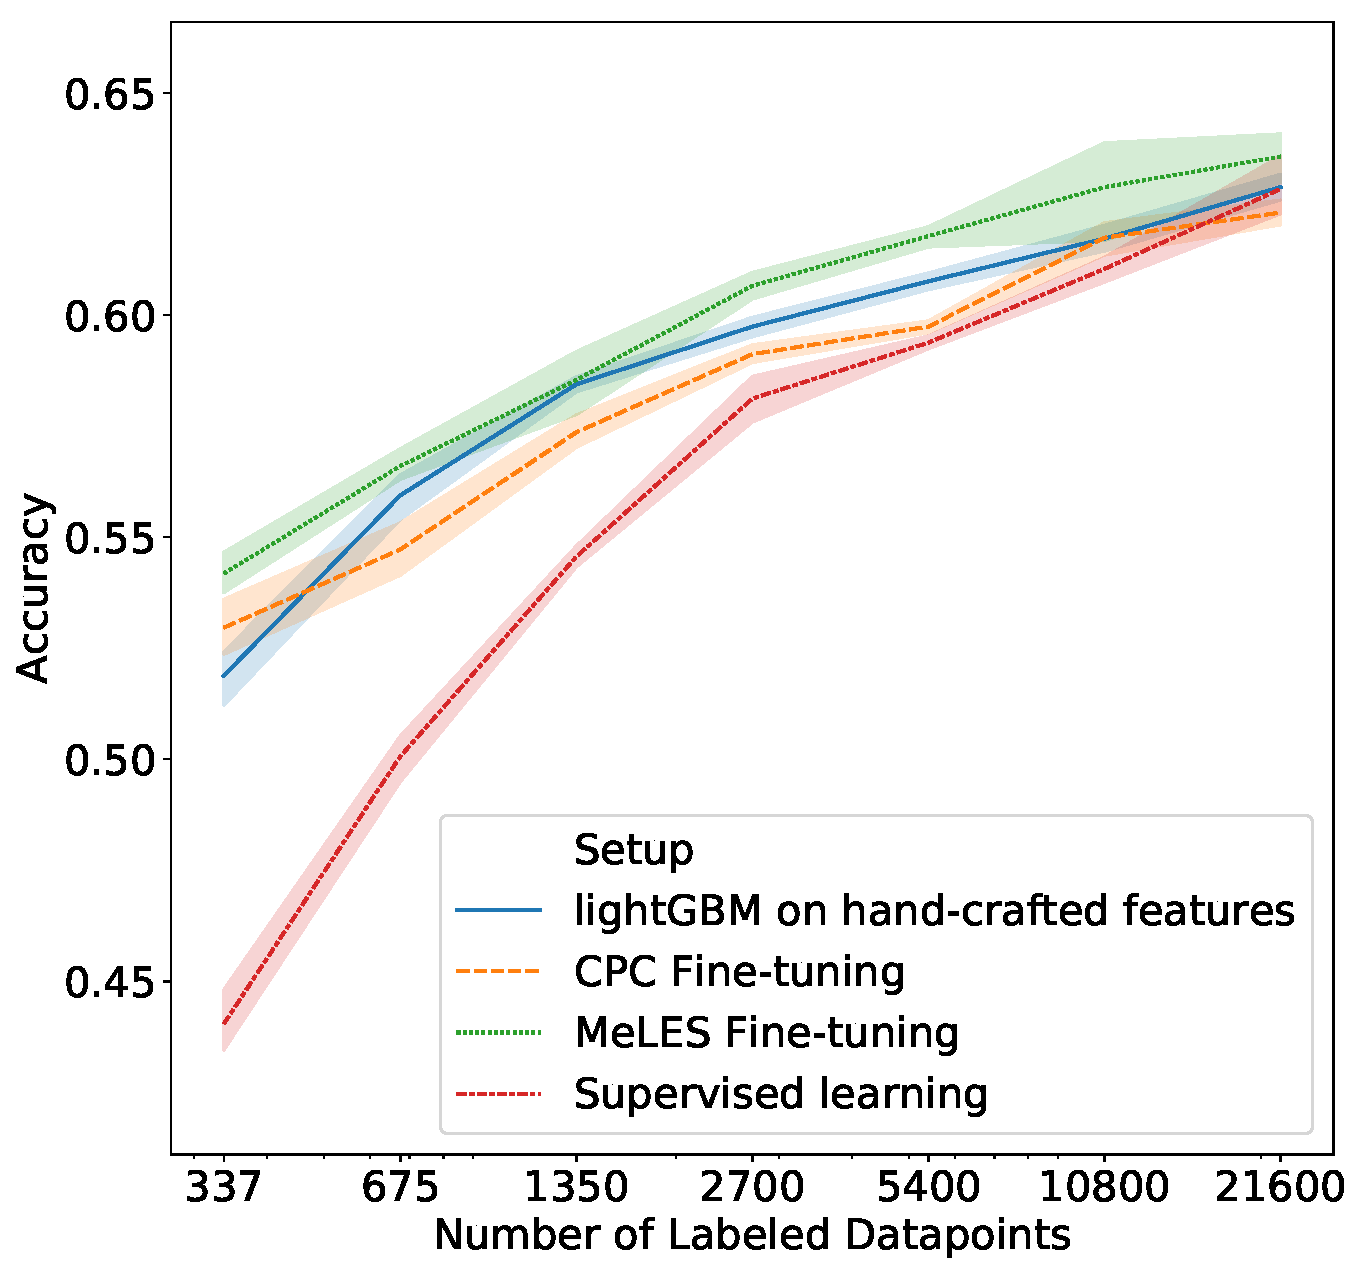
\includegraphics[width=\linewidth]{figures/ss_age_pred.pdf}
    \label{fig-semi-age-0}
  \end{subfigure}%
  \begin{subfigure}{0.5\linewidth}
    \caption{Gender prediction}
    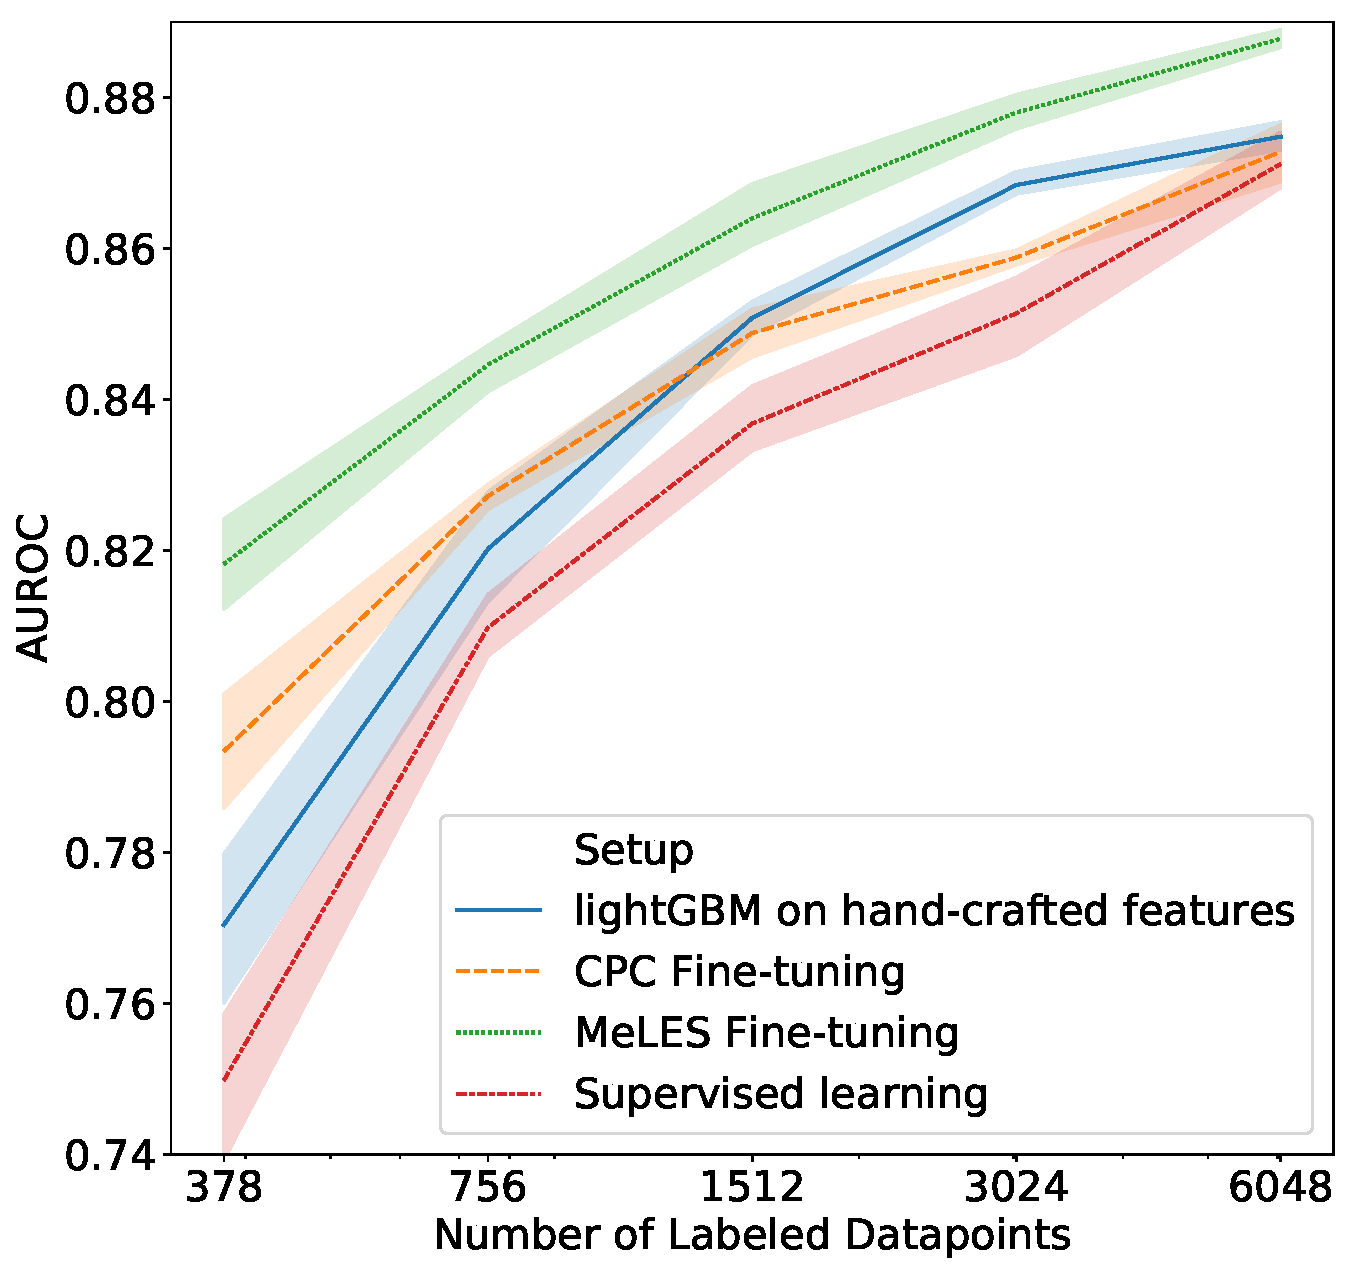
\includegraphics[width=\linewidth]{figures/ss_gen_4.pdf}
    \label{fig-semi-gender-0}
  \end{subfigure}
  \begin{subfigure}{0.5\linewidth}
    \caption{Assessment}
    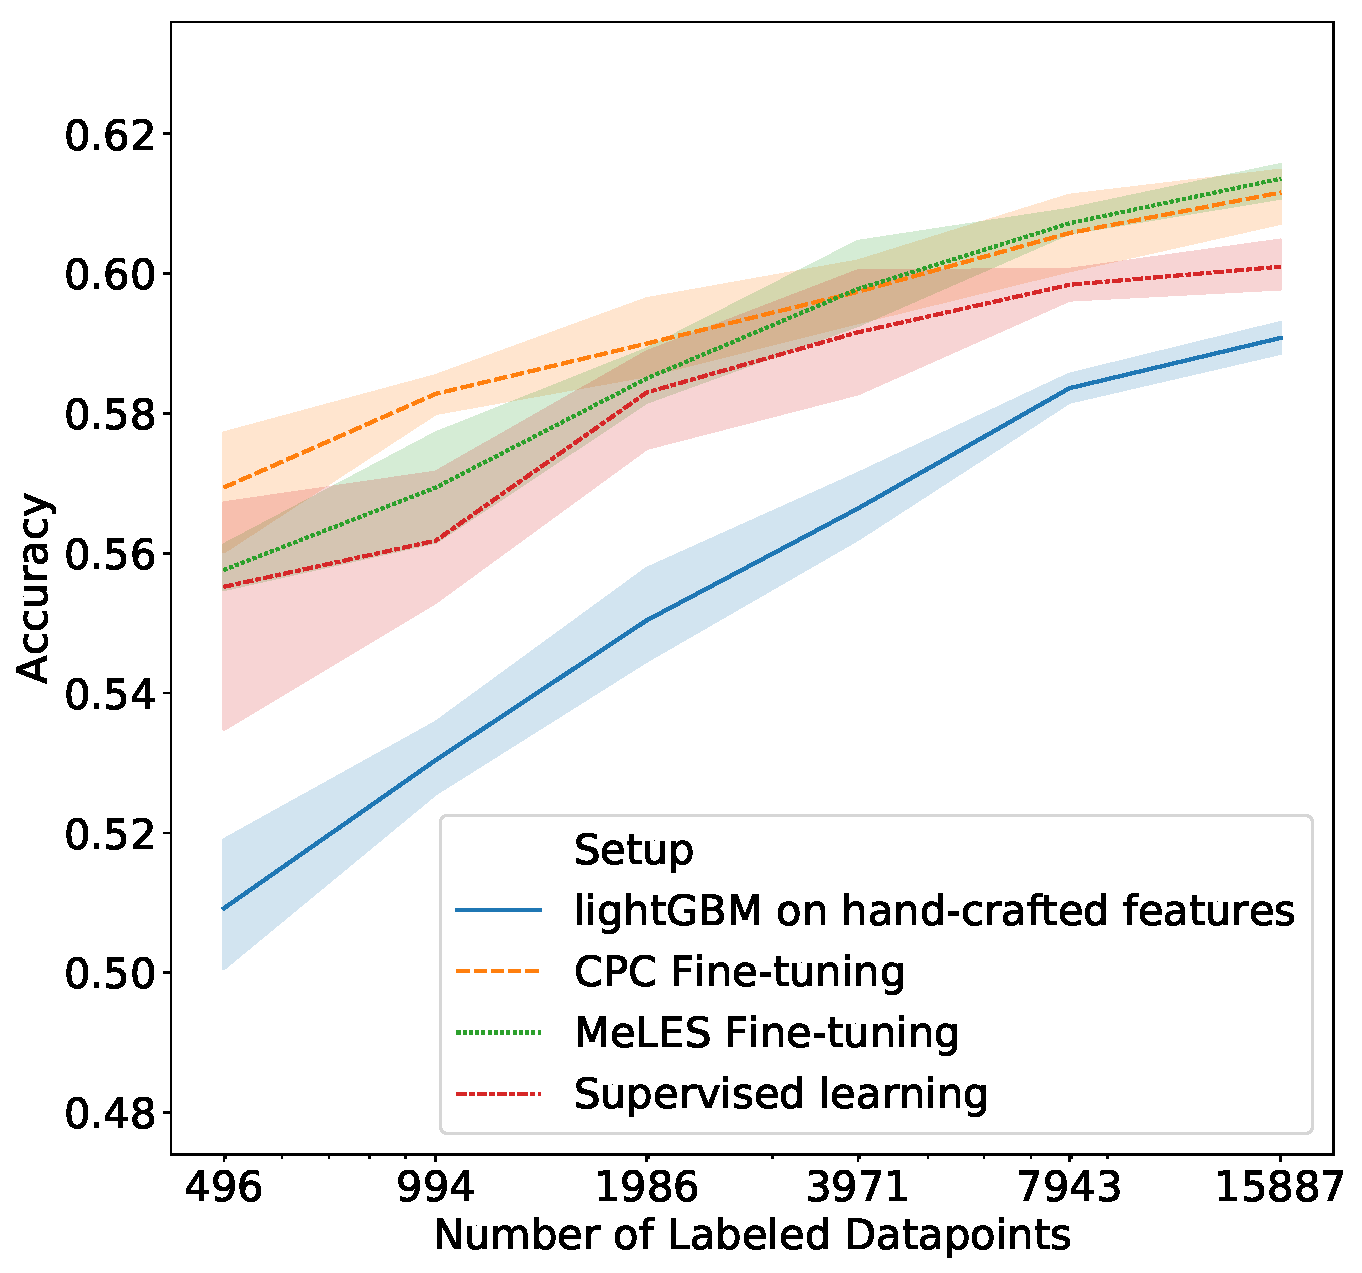
\includegraphics[width=\linewidth]{figures/ss_assessment.pdf}
    \label{fig-semi-age-1}
  \end{subfigure}%
  \begin{subfigure}{0.5\linewidth}
    \caption{Retail}
    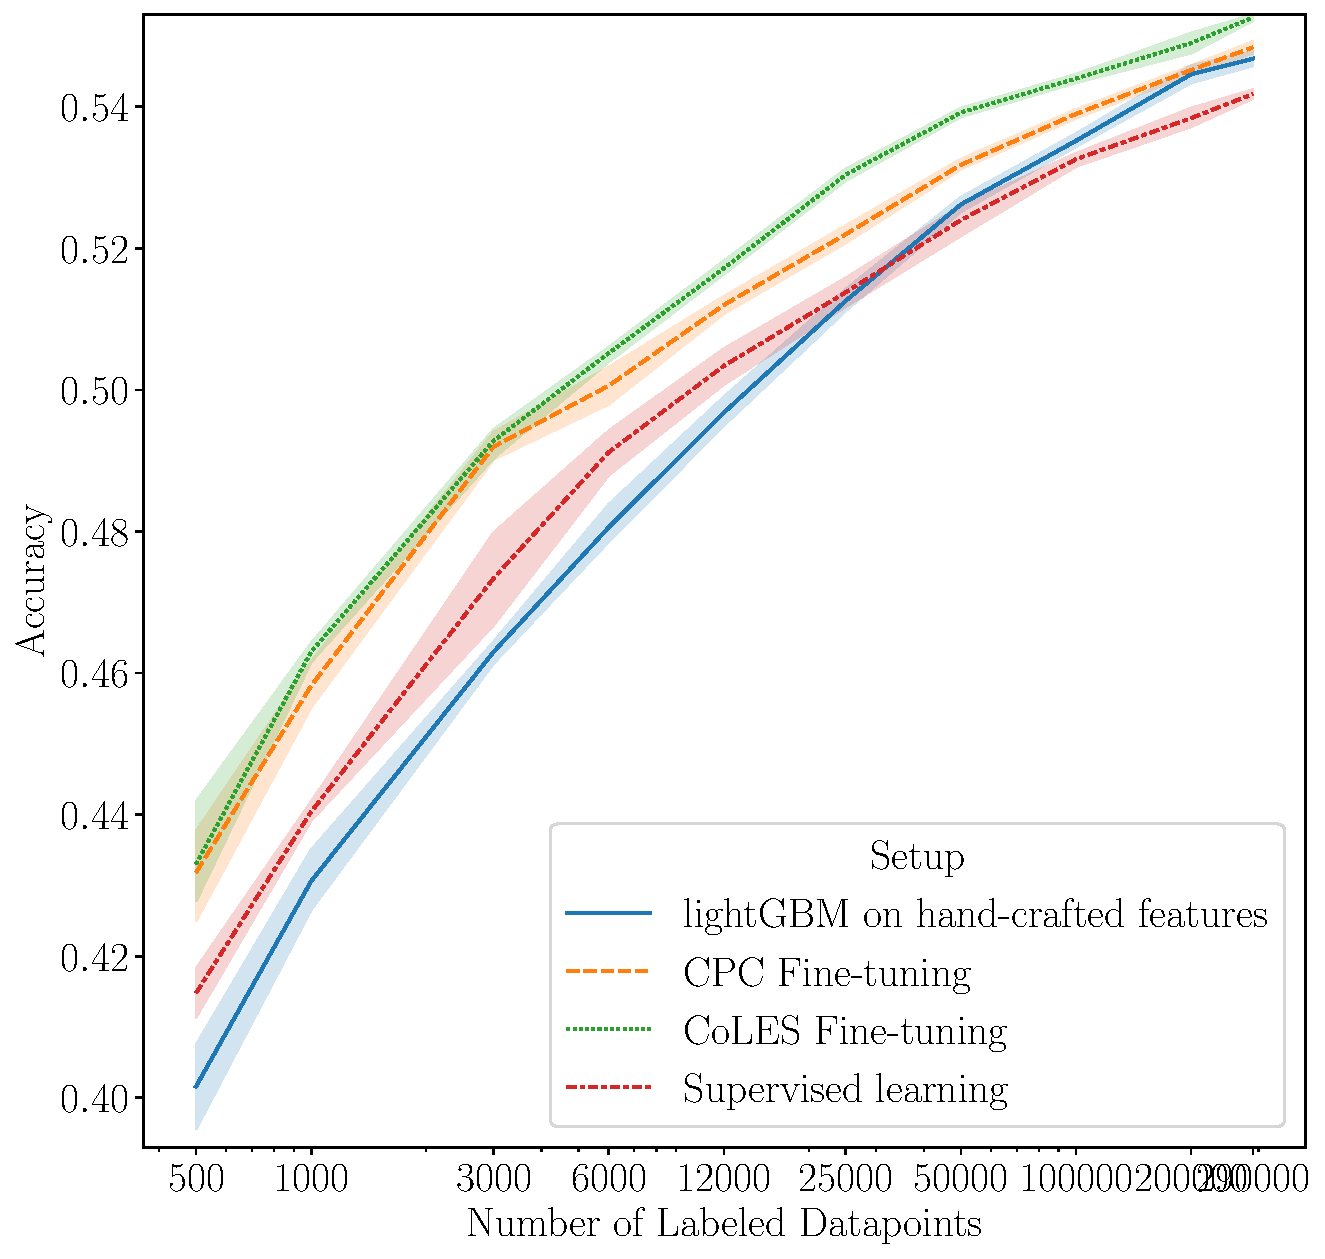
\includegraphics[width=\linewidth]{figures/ss_x5.pdf}
    \label{fig-semi-gender-1}
  \end{subfigure}
  \caption{Model quality for different dataset sizes} \small{The rightmost point correspond to all labels and supervised setup. X-axis is shown on a logarithmic scale.}
  \label{fig-semi}
\end{figure}

\subsection{Embedding visualization}

In order to visualize MeLES embeddings in 2-dimensional space, we applied tSNE transformation~\cite{Maaten2008VisualizingDU} on them. tSNE transforms high-dimensional space to low-dimensional based on local relationships between points, so neighbour vectors in high-dimensional embedding space are pushed to be close in 2-dimensional space. We colorized 2-dimensional vectors using the target values of the datasets.

Note, that embeddings was learned in a fully self-supervised way from raw user transactions without any target information. Sequence of transactions represent user' behavior, thus the MeLES model captures behavioral patterns and outputs embeddings of users with similar patterns nearby.
As shown below, local clusters in embedding space correspond to distribution of user's attributes either age or gender.

tSNE vectors from the age prediction dataset are presented in the Figure \ref{fig-tsne-age2}. We can observe 4 clusters: clusters for group '1' and '2' are on the opposite side of the cloud, clusters for groups '2' and '3' are in the middle.

Taking into account that age is an ordinal attribute, we can make an assumption about the ordering of age groups: $age(1) < age(3) < age(0) < age(2)$ or vice versa. ($age(bin)$ returns age of user for specific group).

tSNE points from gender prediction dataset are presented in the Figure \ref{fig-tsne-gender2}. There are areas dominated by one gender label over another.

\begin{figure}
  \centering
  \caption{2D tSNE mapping of MeLES embeddings colored by target labels}
  \begin{subfigure}{0.5\textwidth}
    \caption{Age prediction}
    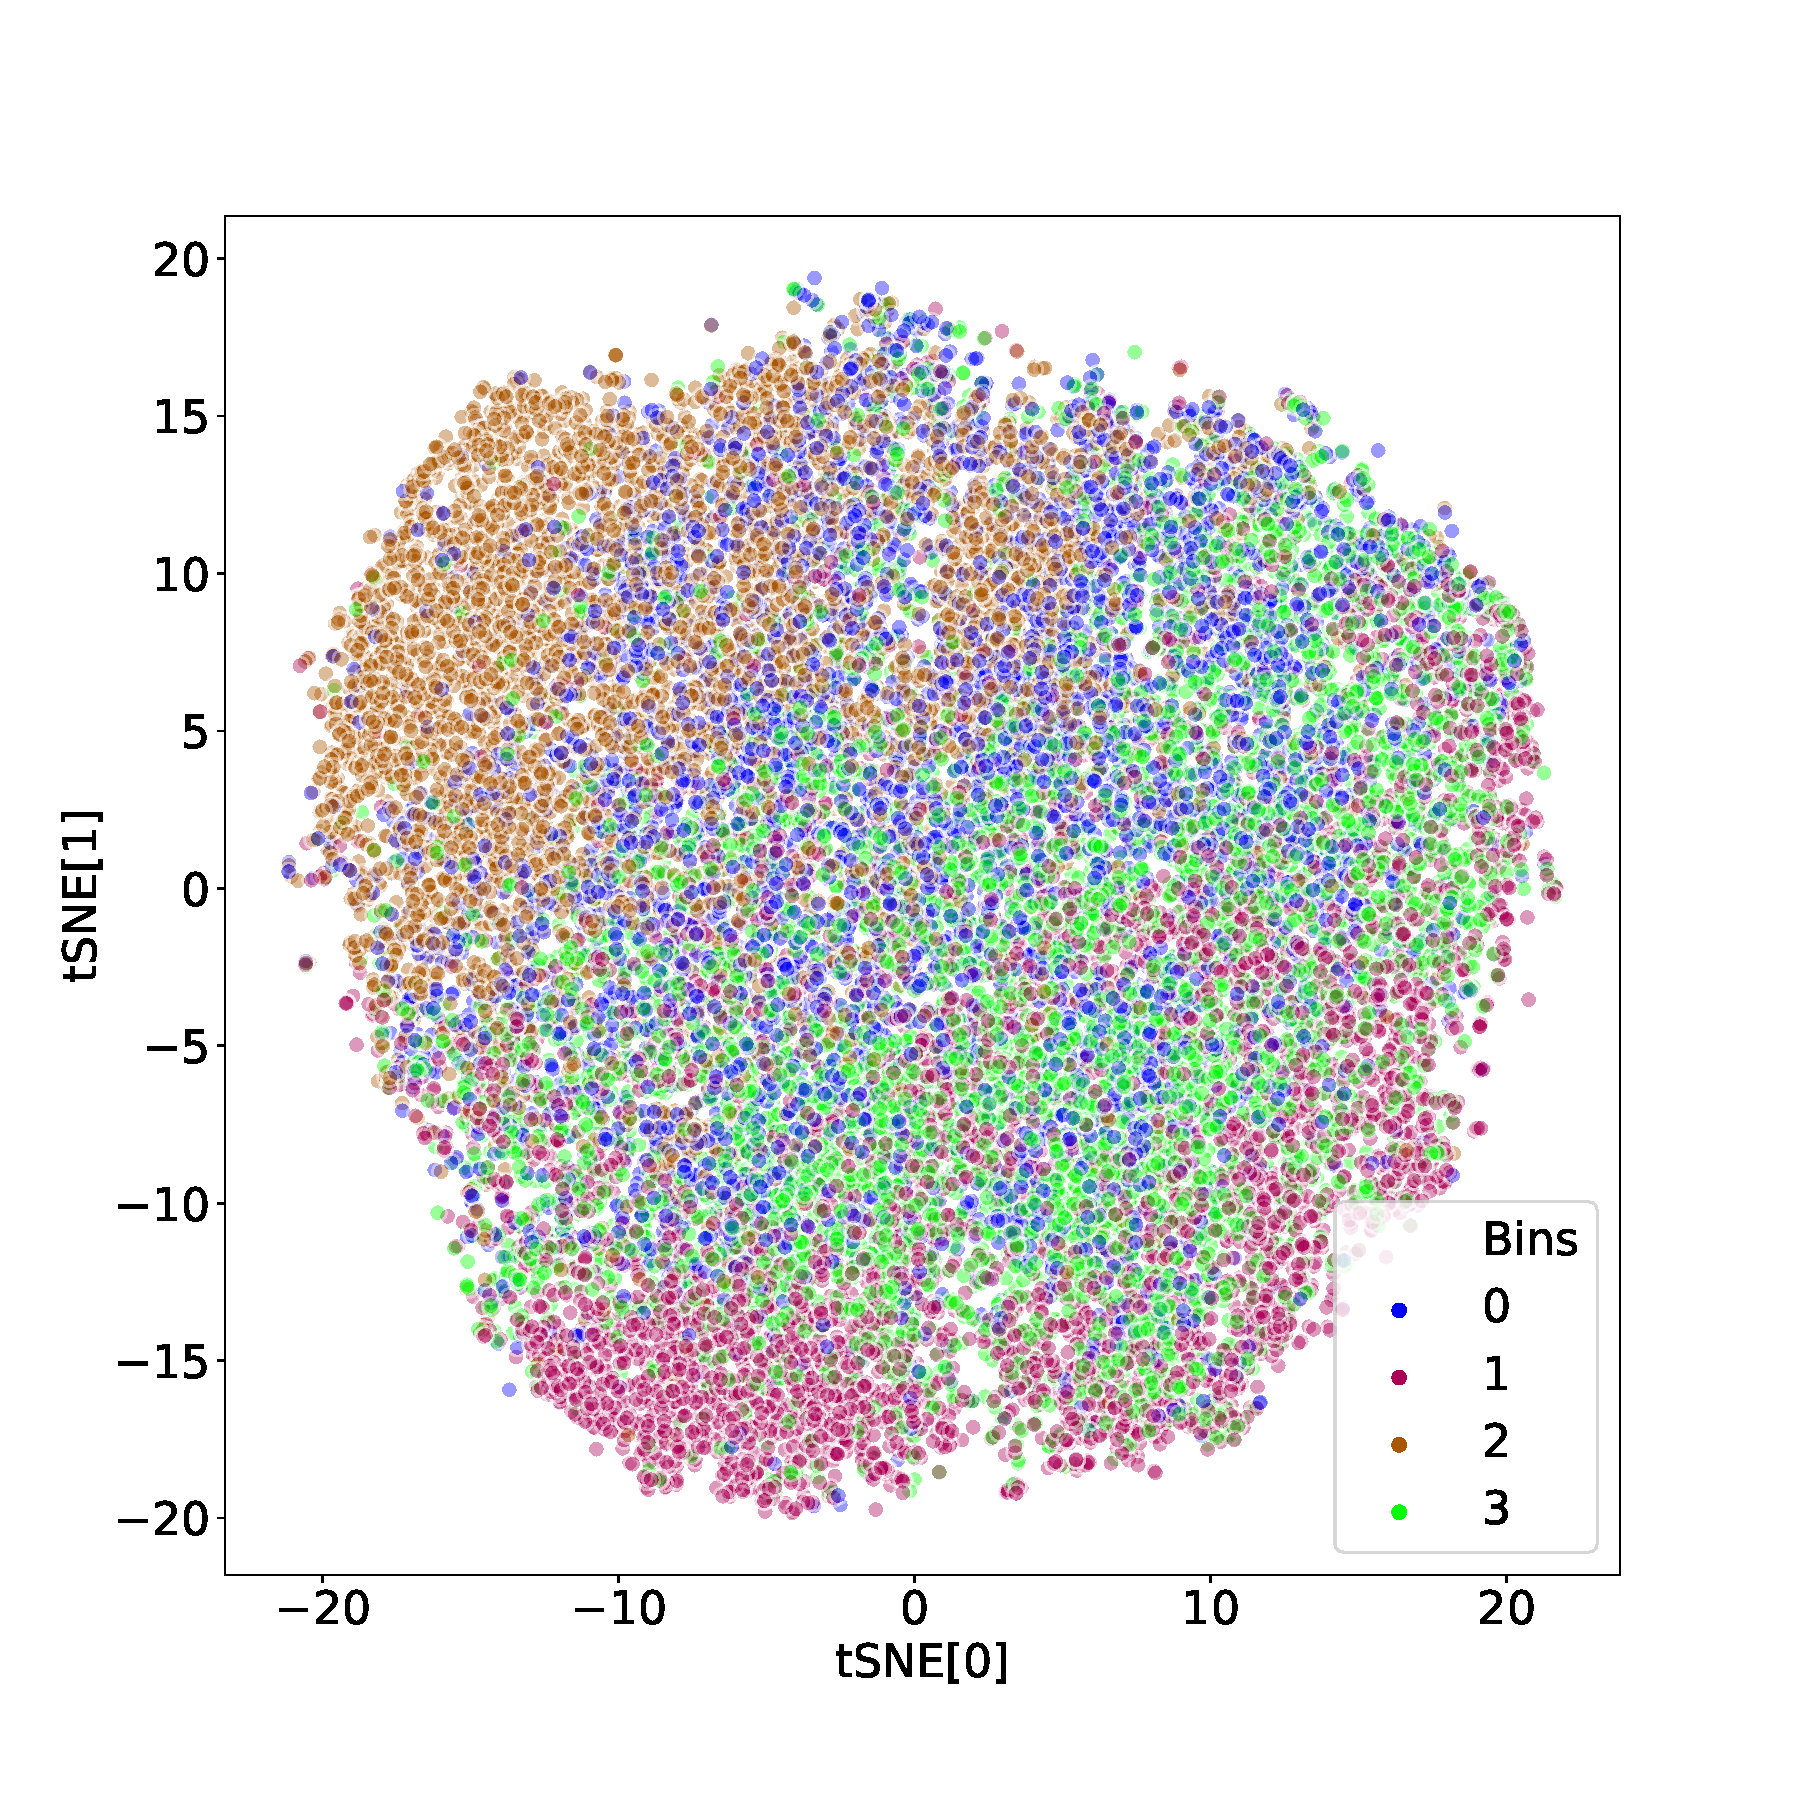
\includegraphics[width=\textwidth]{figures/age-pred-tsne2.pdf}
    \label{fig-tsne-age2}
  \end{subfigure}%
  \begin{subfigure}{0.5\textwidth}
    \caption{Gender prediction}
    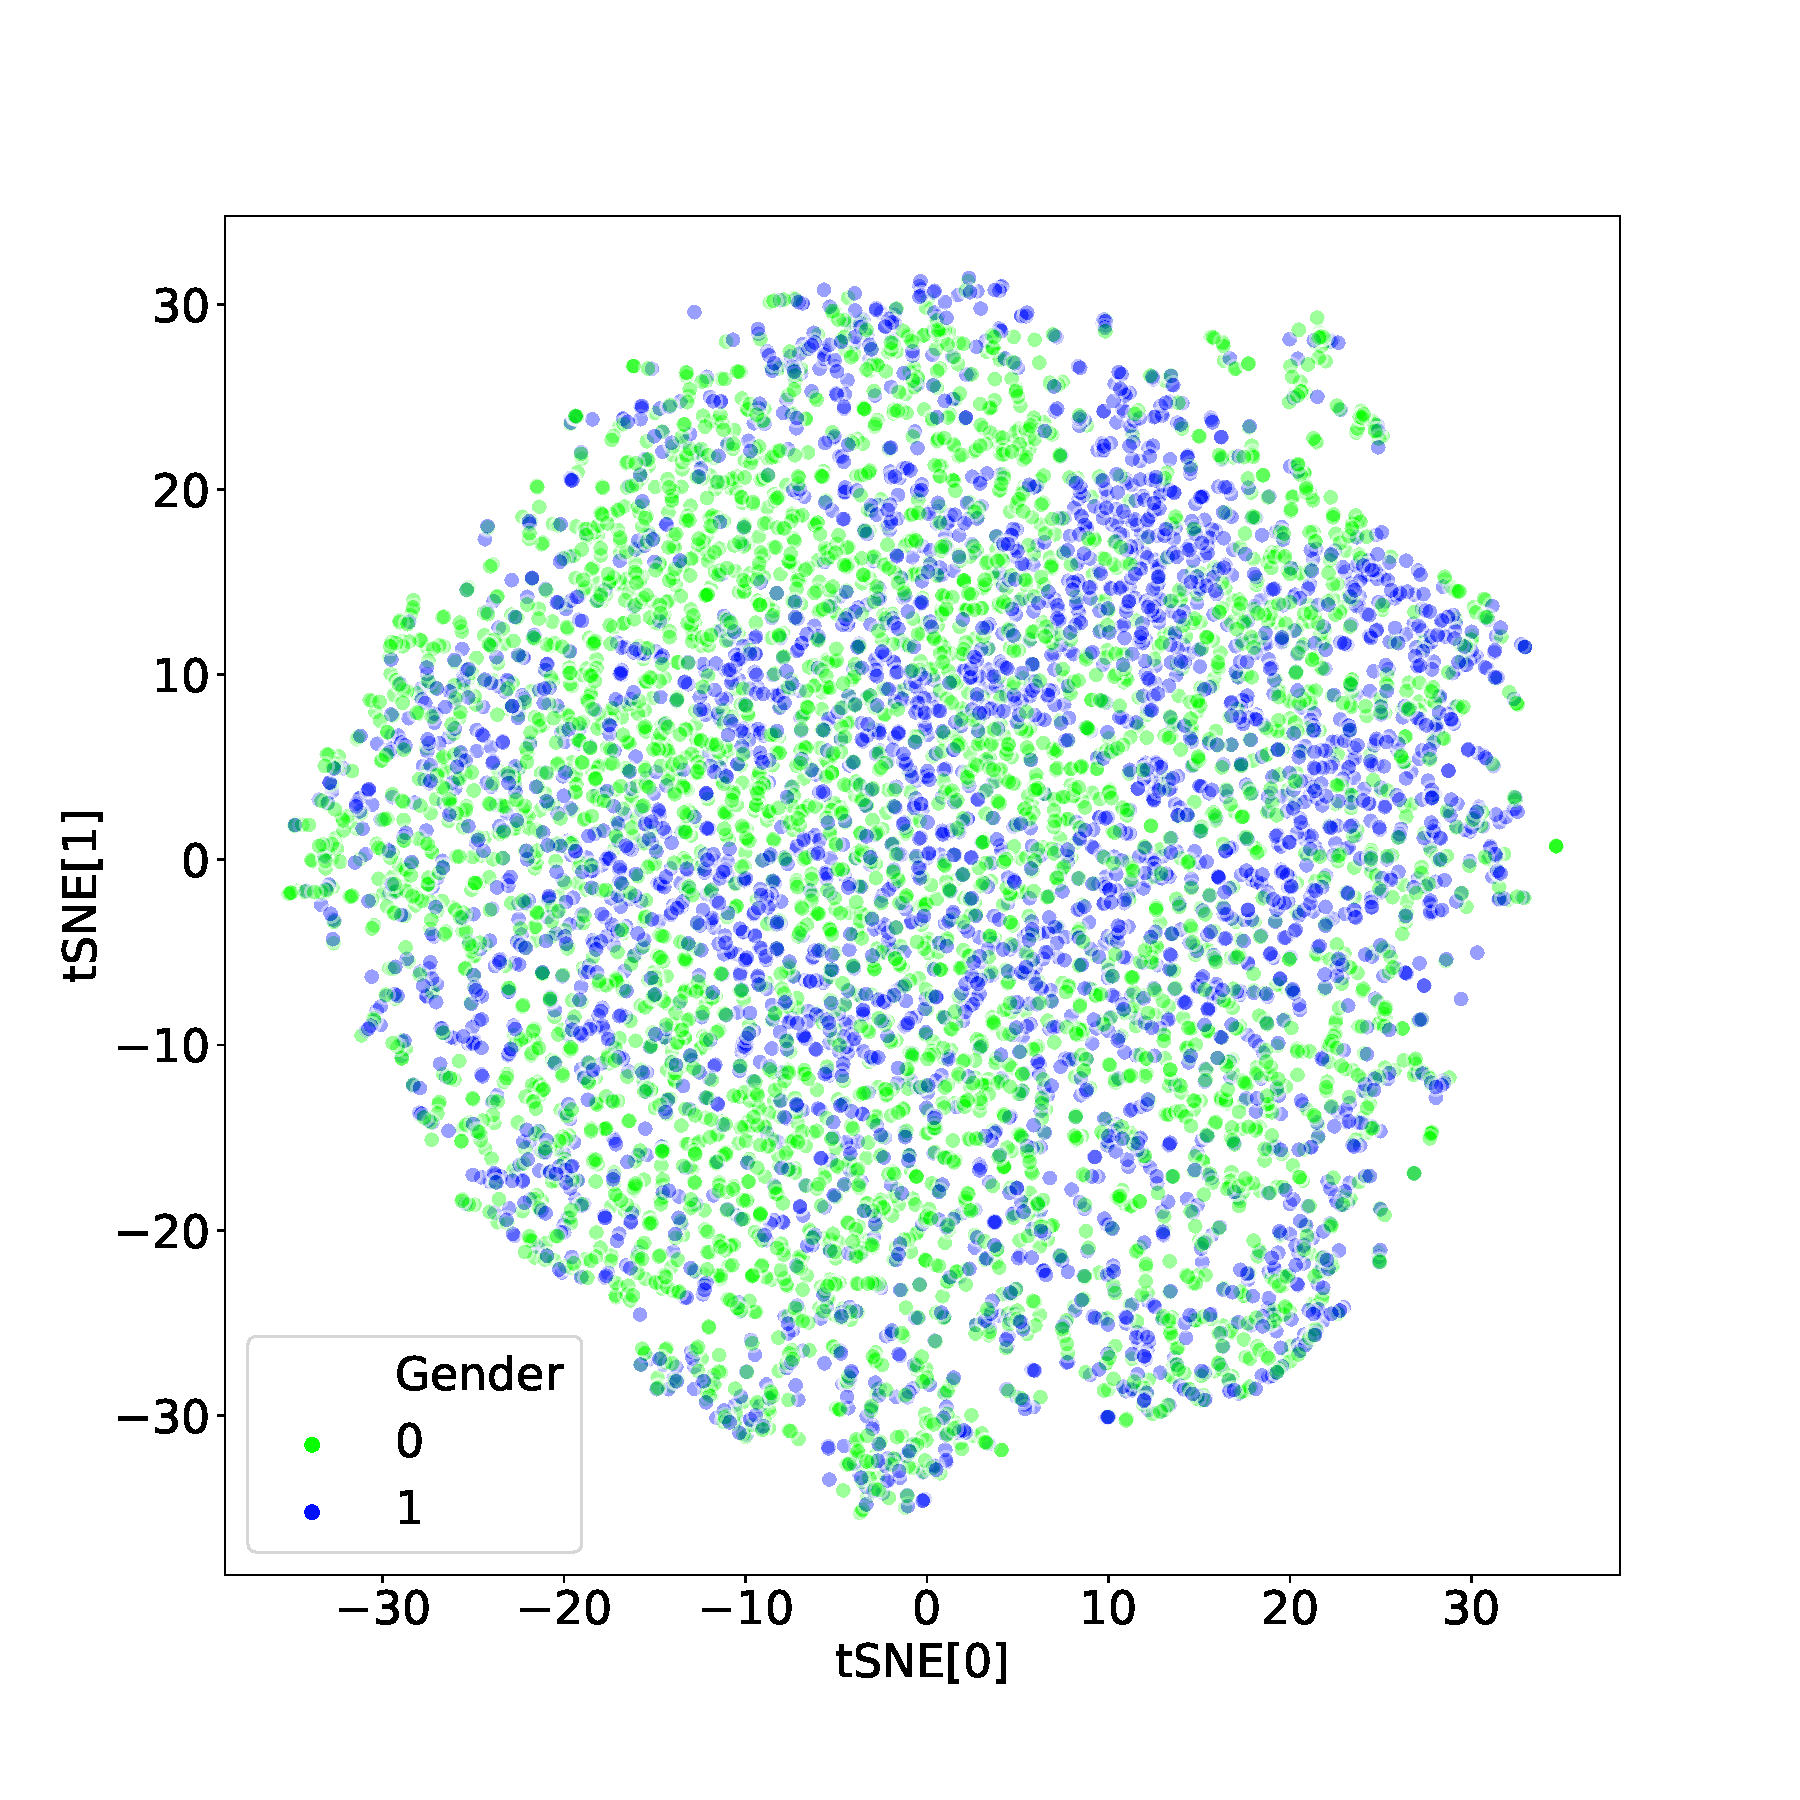
\includegraphics[width=\textwidth]{figures/gender-tsne2.pdf}
    \label{fig-tsne-gender2}
  \end{subfigure}

  \begin{subfigure}{0.5\textwidth}
    \caption{Assessment}
    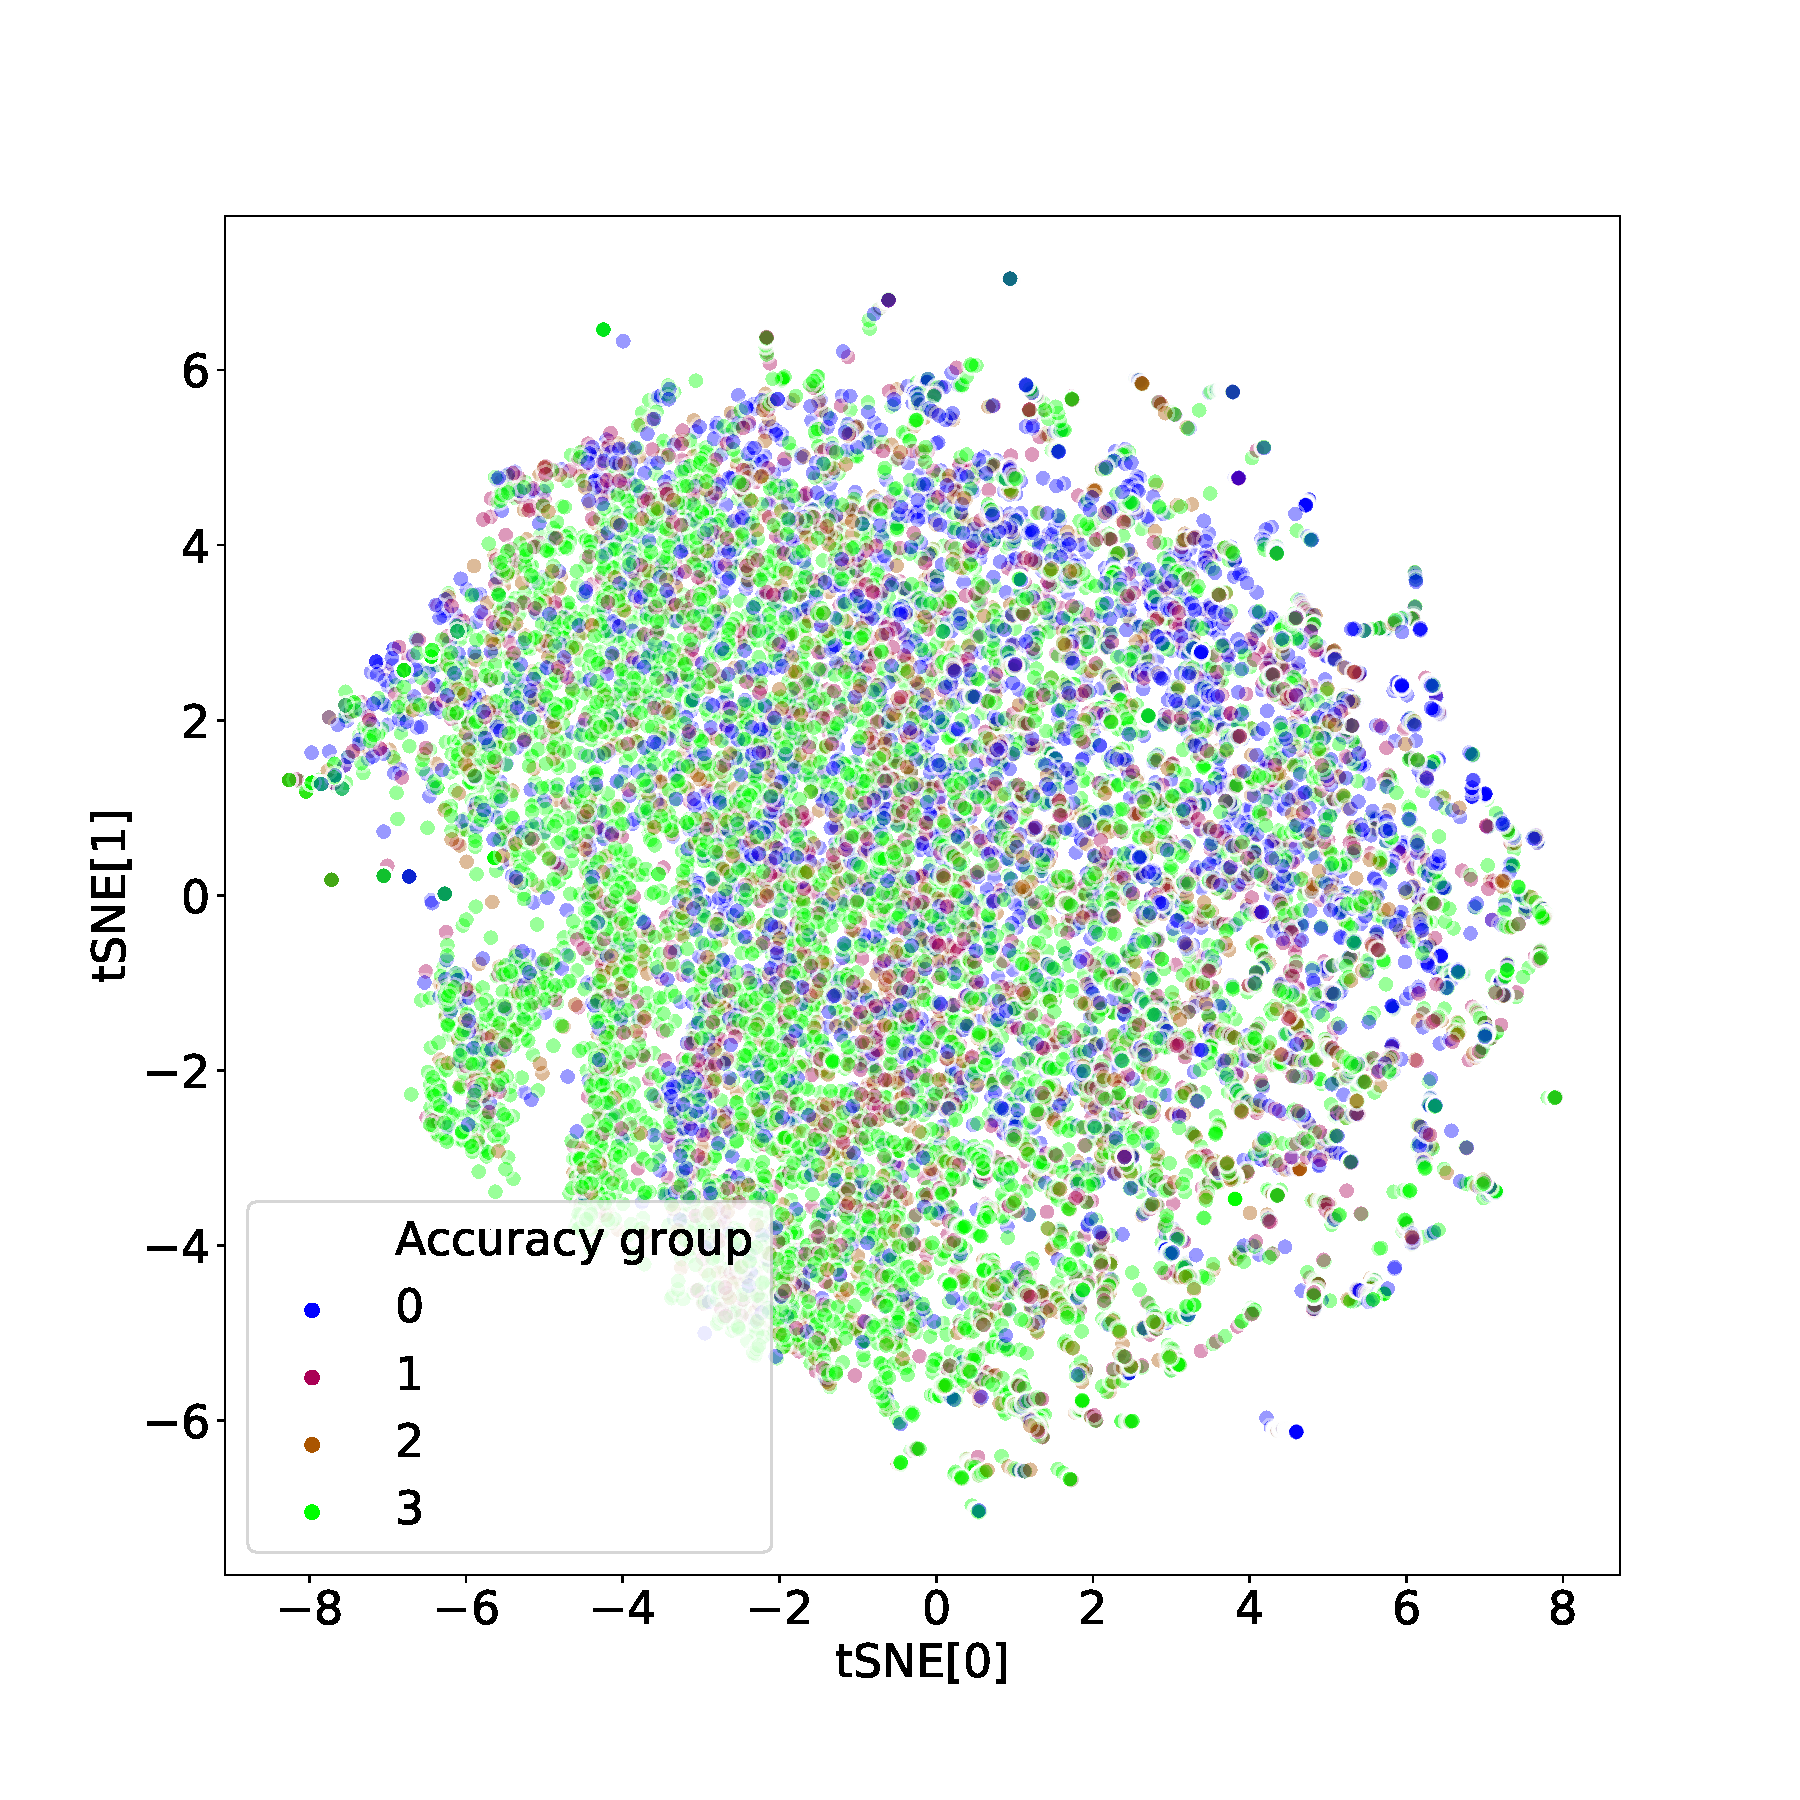
\includegraphics[width=\textwidth]{figures/bowl-tsne-accuracy_group.pdf}
    \label{fig-tsne-bowl}
  \end{subfigure}%
  \begin{subfigure}{0.5\textwidth}
    \caption{Retail}
    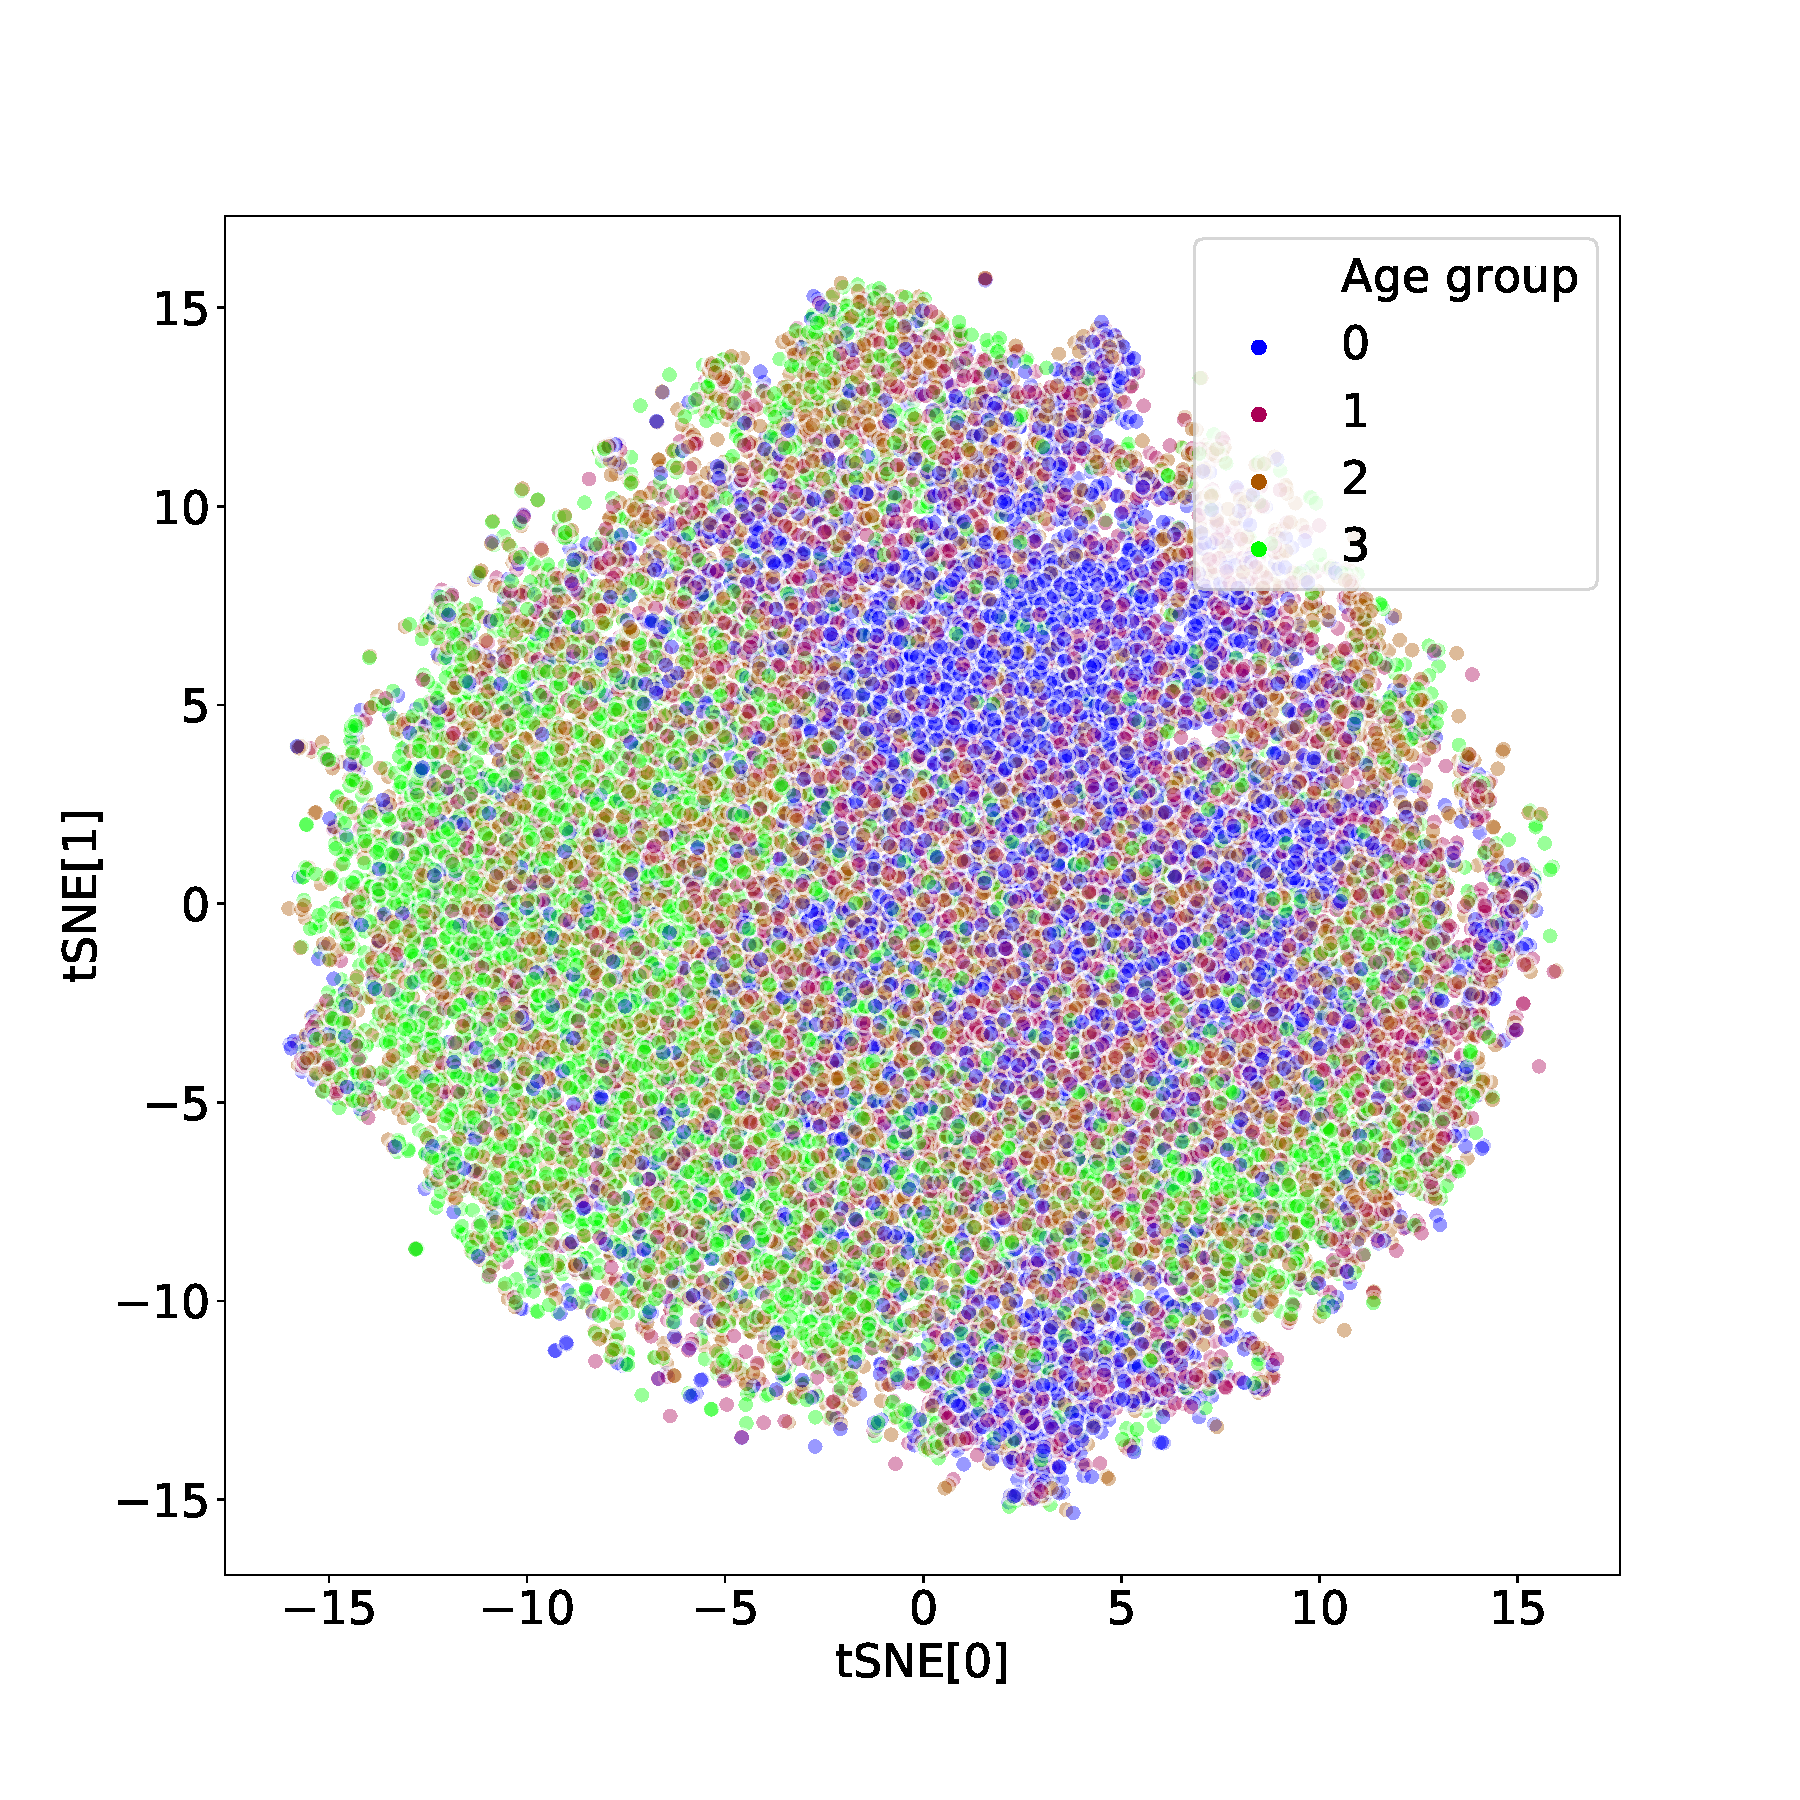
\includegraphics[width=\textwidth]{figures/x5-tsne-age_bin.pdf}
    \label{fig-tsne-x5}
  \end{subfigure}
\end{figure}

\bibliographystyle{humannat}
\bibliography{neurips2020}

\end{document}